\documentclass{article}

\usepackage{verbatim}
\usepackage{minted}
\usepackage{graphicx}

\title{Langages synchrones : TP2}

% A rendre le 04/11
% Metronome: 1,2,3,6
% Arbitre McMillan: 1,2
% Extensions: Q1 (non determinism), Q2 (asynchronisme)

%ssh 3367424@ssh.ufr-info-p6.jussieu.fr

\author{I\~{n}igo Mediavilla \& Pierrick Couderc}

\begin{document}

\maketitle

\section{Métronome}

\subsection{Noeud Lustre}

\begin{verbatim}
node metronome (reset : bool; delay : int) 
     returns (tic, tac : bool);
  var n, hz : int;
      state, first, tmp: bool;
let
    hz = 0 -> if reset then delay - 1 else pre hz;
    n = 0 -> if reset then delay
             else if pre n = 0 and first then hz
             else (pre n) - 1;
    first = false -> reset or pre first;
    state = n = 0 and first;

    tmp = true -> if state then not pre tmp else pre tmp;
    
    tic = if state then tmp else false;
    tac = if state then not tmp else false;
tel
\end{verbatim}


In the figure~\ref{trace-metronome-1} we can see how the given code
emulates the behaviour of the metronome. In the step 6, we set a
delay of 1 and we verify that the metronome emits tics and tacs
alternatively. In the step 13 we modify the delay to 5 and we not
only see how this delay is respected but also how the next signal
emitted is not tic but tac, since the last sinal emmited with delay
1 was tic.

\subsection{Automaton}

The code for C for the metronome that is generated with the commands
lus2oc and poc is shown in figure~\ref{metronome-0}.

\begin{figure}[ht]

\begin{minted}[mathescape,
               linenos,
               numbersep=5pt,
               gobble=2,
               frame=lines,
               framesep=2mm]{c}
  switch(ctx->current_state){
   case 0:
      ctx->_V5 = (ctx->_V3? _false : (ctx->_V1 || ctx->_V5));
      ctx->_V6 = (ctx->_V3? 0 : (ctx->_V1? (ctx->_V2 - 1) : ctx->_V6));
      ctx->_V4 = (ctx->_V3? 0 : (ctx->_V1? ctx->_V2 : (((ctx->_V4 == 0) &&
   ctx->_V5)? ctx->_V6 : (ctx->_V4 - 1))));
      ctx->_V10 = ((ctx->_V4 == 0) && ctx->_V5);
      ctx->_V7 = (ctx->_V3? _true : (ctx->_V10? (!ctx->_V7) : ctx->_V7));
      ctx->_V3 = _false;
      ctx->_V8 = (ctx->_V10? ctx->_V7 : _false);
      metronome_O_tic(ctx->client_data, ctx->_V8);
      ctx->_V9 = (ctx->_V10? (!ctx->_V7) : _false);
      metronome_O_tac(ctx->client_data, ctx->_V9);
      ctx->current_state = 0; break;
   break;
   } /* END SWITCH */
\end{minted}
\label{metronome-0}
\caption{Code C generated with with lus2oc -0 and poc}
\end{figure}

The correspondance of the variables in the C code with
respect to the code in lustre is the following:

\begin{itemize}
\item V1 = reset
\item V2 = delay
\item V3 = initial state = false
\item V4 = n              
\item V5 =          
\item V6 = hz
\item V7 = tmp               
\item V8 = tic  
\item V9 = tac
\item V10 = state
\end{itemize}

And thus the corresponding automaton for the C code is shown
in figure~\ref{automaton-0}

\begin{figure}[!ht]
\begin{center}
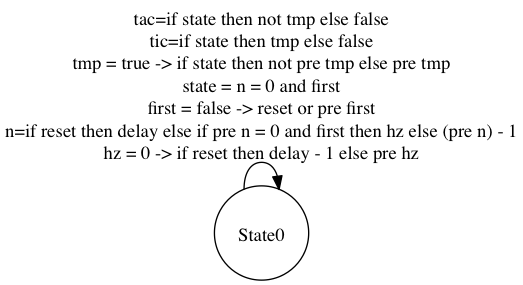
\includegraphics[width=0.8\textwidth, natwidth=610,natheight=642] {automaton-0.png}
\end{center}
\label{automaton-0}
\caption{Automaton without unfolding}
\end{figure}

If we generate the automaton with the option -2, the automaton
is unfolded so the only state that we had for the option -0, is
converted into 4 states. As demonstrated by figure~\ref{automaton-2}
the automaton is unfolded based on the values of the signals \emph{reset}
and \emph{state}.

\begin{figure}[!ht]
\label{automaton-2}
\caption{Automaton with unfolding}
\begin{center}
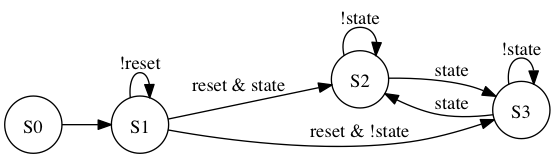
\includegraphics[width=0.8\textwidth, natwidth=610,natheight=642]{automaton-2.png}
\end{center}
\end{figure}

The way it works:

priority : cell 3 > cell2 > cell1 

In equal circumstances the one that has the priority gets the ack, however
if one cell that keeps requesting gets the token twice it means that it has waited
for the whole cycle so its time for it to get the ack. (this way avoiding deadlock)

- When there's only one of them that is requesting then it gets the ack all the time

all-req-1

- When there's two that request separately, they don't conflict so the one that
demands always get the ack

two-alternate

- When there's two of them that request continuosly, then one gets two turns and 
the other gets one turn out of three

- When there's the three requests at the same time, the third cell always takes the
token because it has priority over the others and since no cell keeps the request
long enough to get twice the token while the request is active, the mecanism to avoid
"famine" doesn't activate.

three-sporadic

- When there's three continuosly that have been waiting waiting for more than one cycle
for the token, the graph shows that the three get the ack alternatively. Every time 
  one gets the ack is because it's because that cell is getting the token

three-continuosly

- In the beginning we can see that the first time we don't have enough info
to calculate the acks so we return false by default even though the three
acks have been activated. The token initially is in cell 1. On the second, third
and fourth steps cell 3 gets the ack because it has priority with respect to cells 
1 and 2. Finally they get back to the behaviour of alternating the ack shown in the
previous example.

Q2 Question 2 : Générez l'automate de l'arbitre (option -2). Combien d'états contient-il, quelles variables ont été dépliées ?

\subsection{McMillan's referee - Automaton}

When generating the automaton with lus2oc and the code with poc we can see how
the code contains 24 states. Every change to a new state is guided by the input
signals req\_in\_1, req\_in\_2 and req\_in\_3. Intuitively we can imagine that
the states have been unfolded based on whether the cells have been waiting for
an ack since the last time they got the token or not and if they have the token
now or not. We can see that if at every step we need to keep for every cell
a boolean value saying if the cell has been waiting for the ack since the last
token then we need $2^{3}$ states just to do that. If on top of that we need
to keep track on where the token is at every moment we need to multiply the 
previous value by three (the token can be in cell1, cell2 or cell3) what
gives us the value of 24 $2^{3}~\times~4~=~24$.

%\begin{figure}
%\label{trace-metronome-1}
%\caption{Execution of the metronome}
%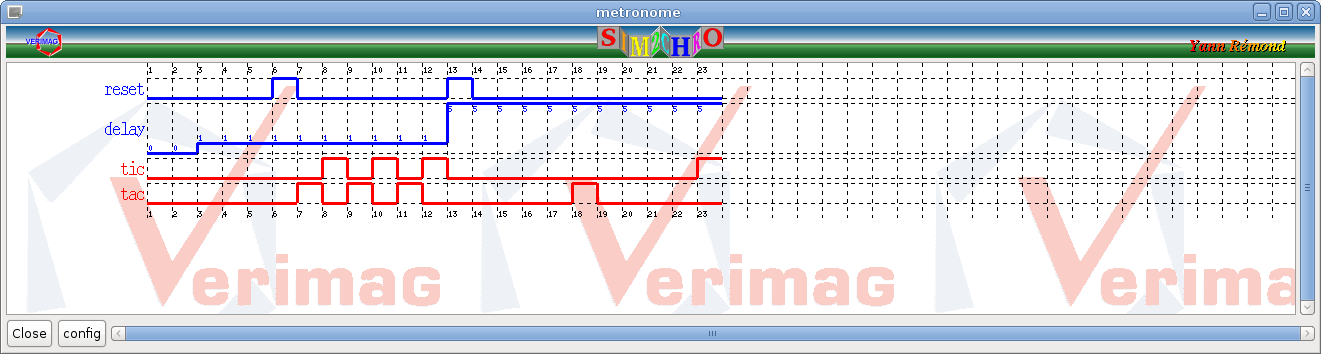
\includegraphics [scale=0.4]{metronome_1.png}
%\end{figure}
\end{document}
